
  \section{Introduction}
This project uses Arduino and various libraries to create a weighing system with an HX711 load cell amplifier, an LCD display, and a tare button. The program continuously reads the change in weight and displays it on both the Serial Monitor and the LCD screen. We also implemented a tare button to reset the scale to zero when needed.



\begin{figure}[H]
    \centering
    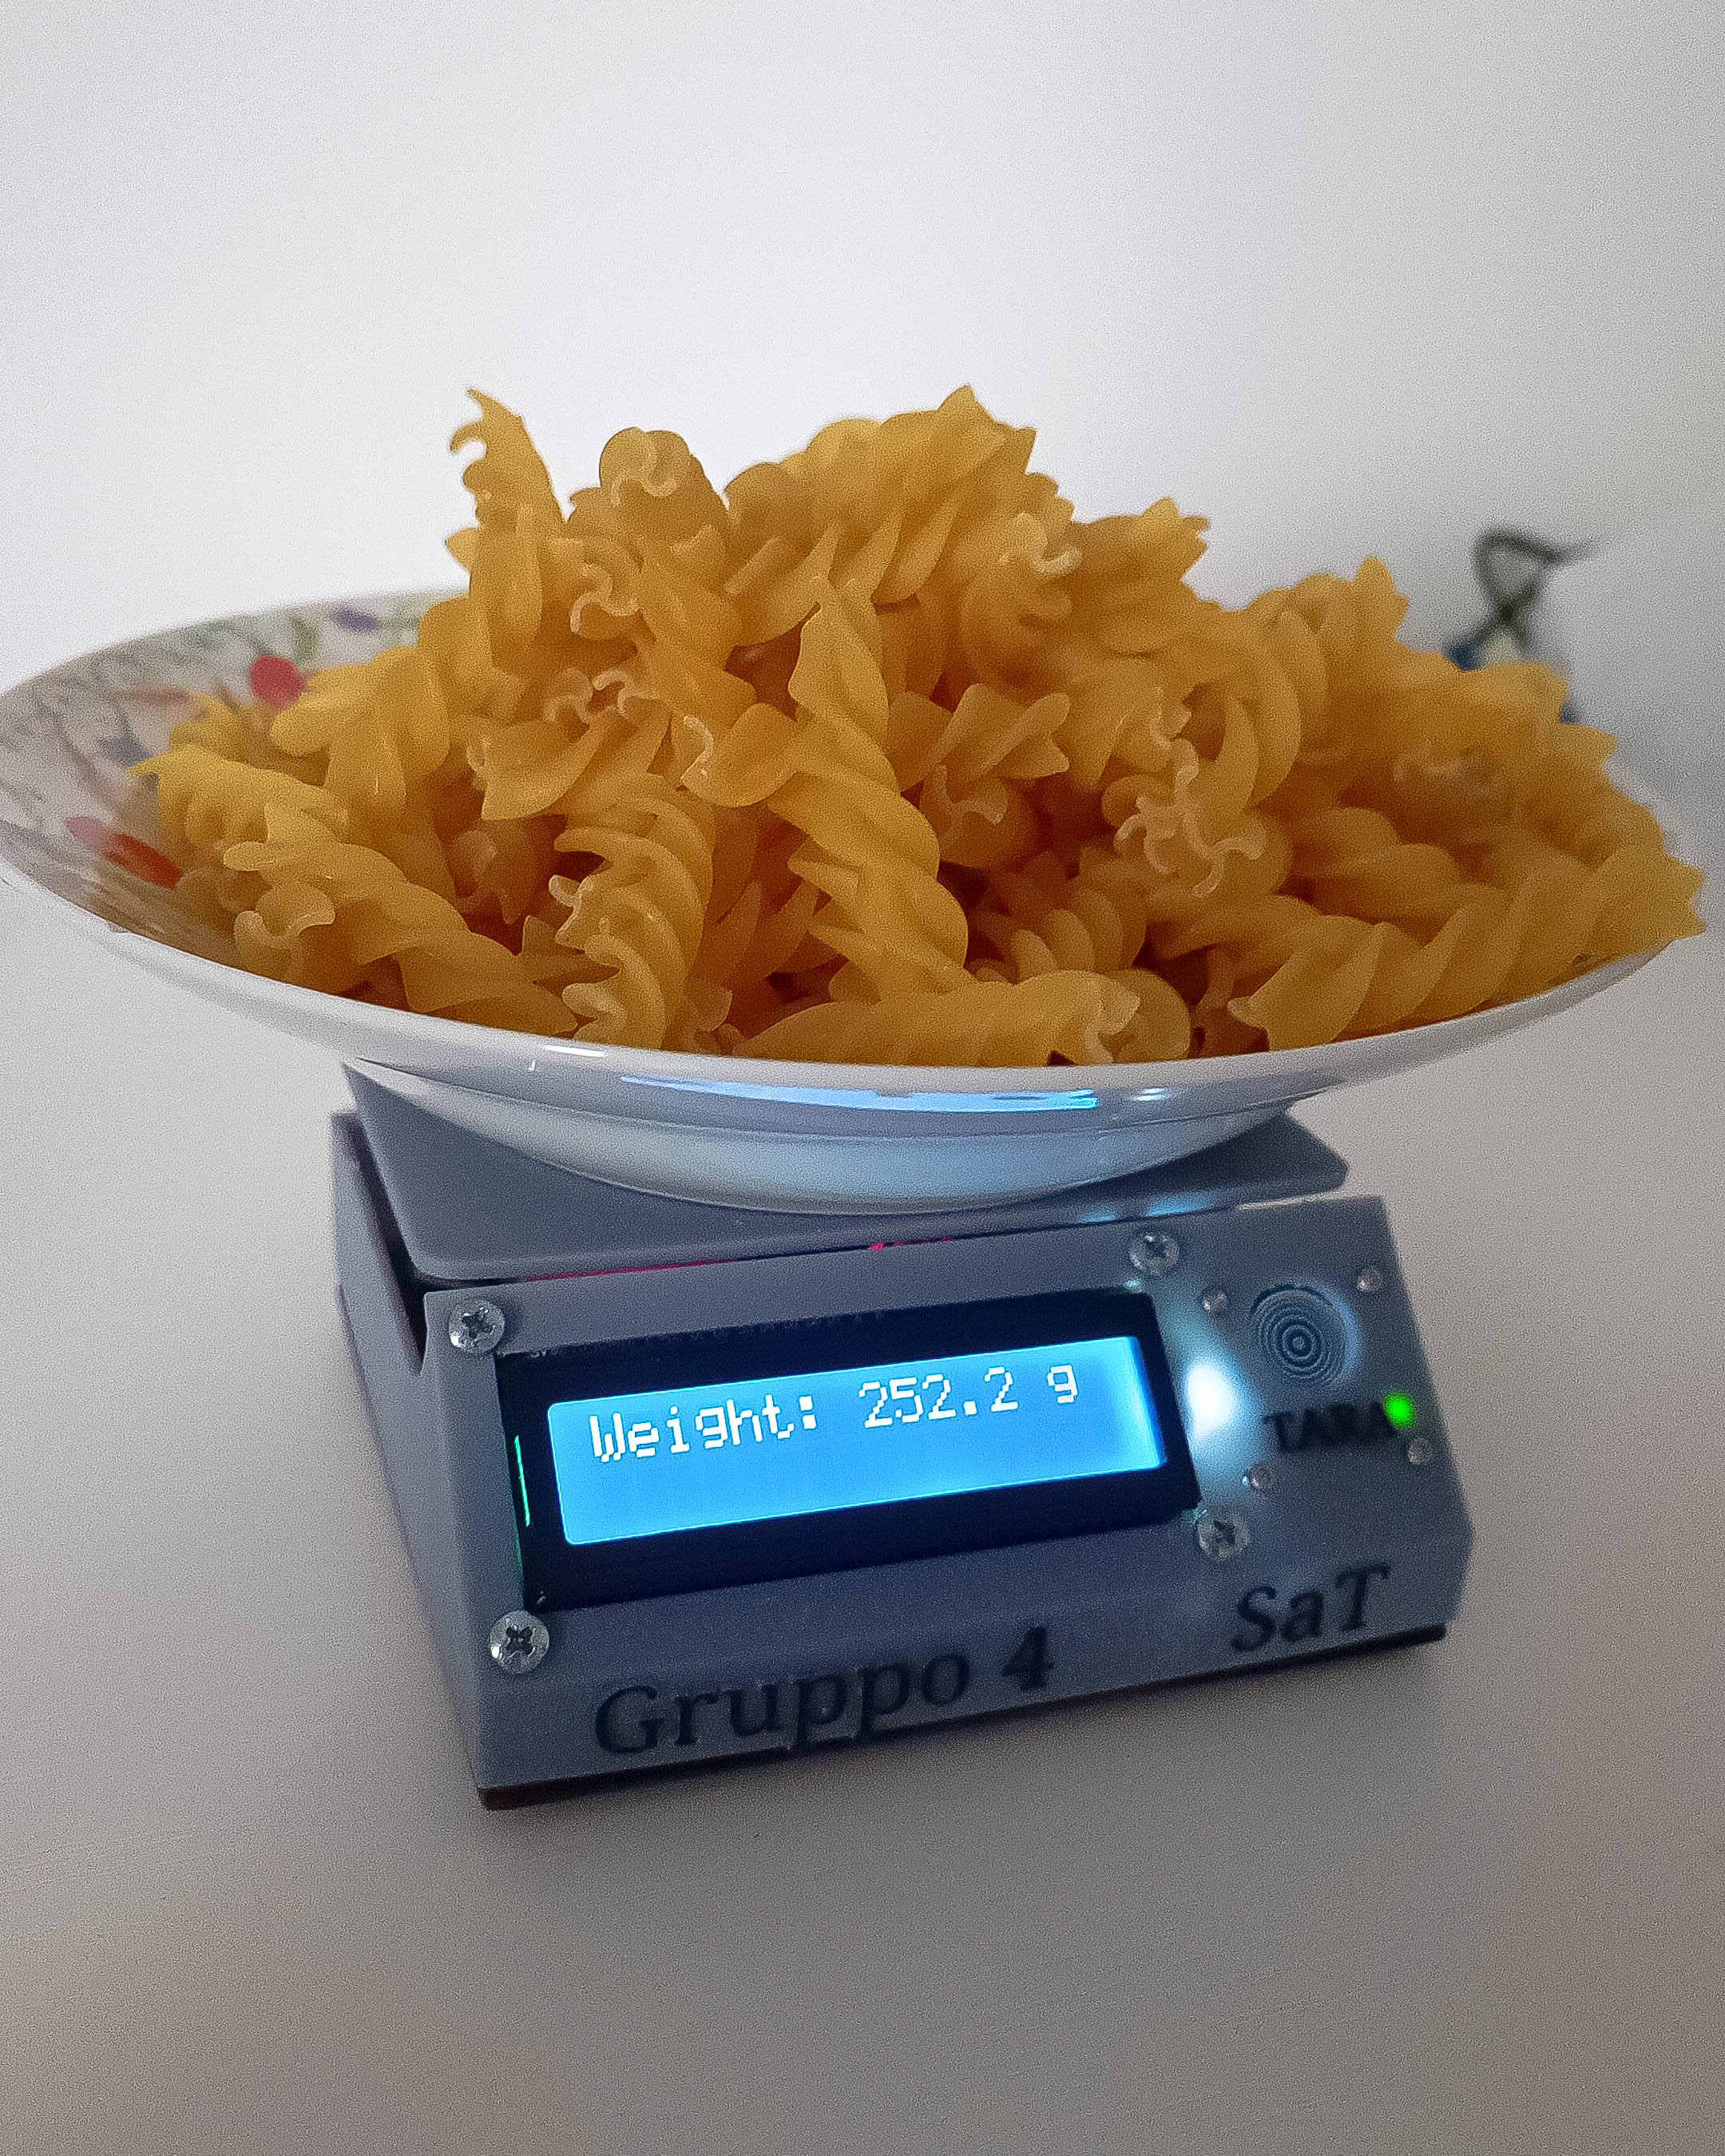
\includegraphics[width=0.8\textwidth]{medias/photos/test1.jpg}
    \caption{Test with some pasta}
    \label{fig:immagine}
\end{figure}

\subsection{Weighting Scale assembly}

Watch the following video:
\url{https://www.youtube.com/watch?v=QM5nMauuca8}

\subsection{Photos}
\begin{figure}[H]
    \centering
    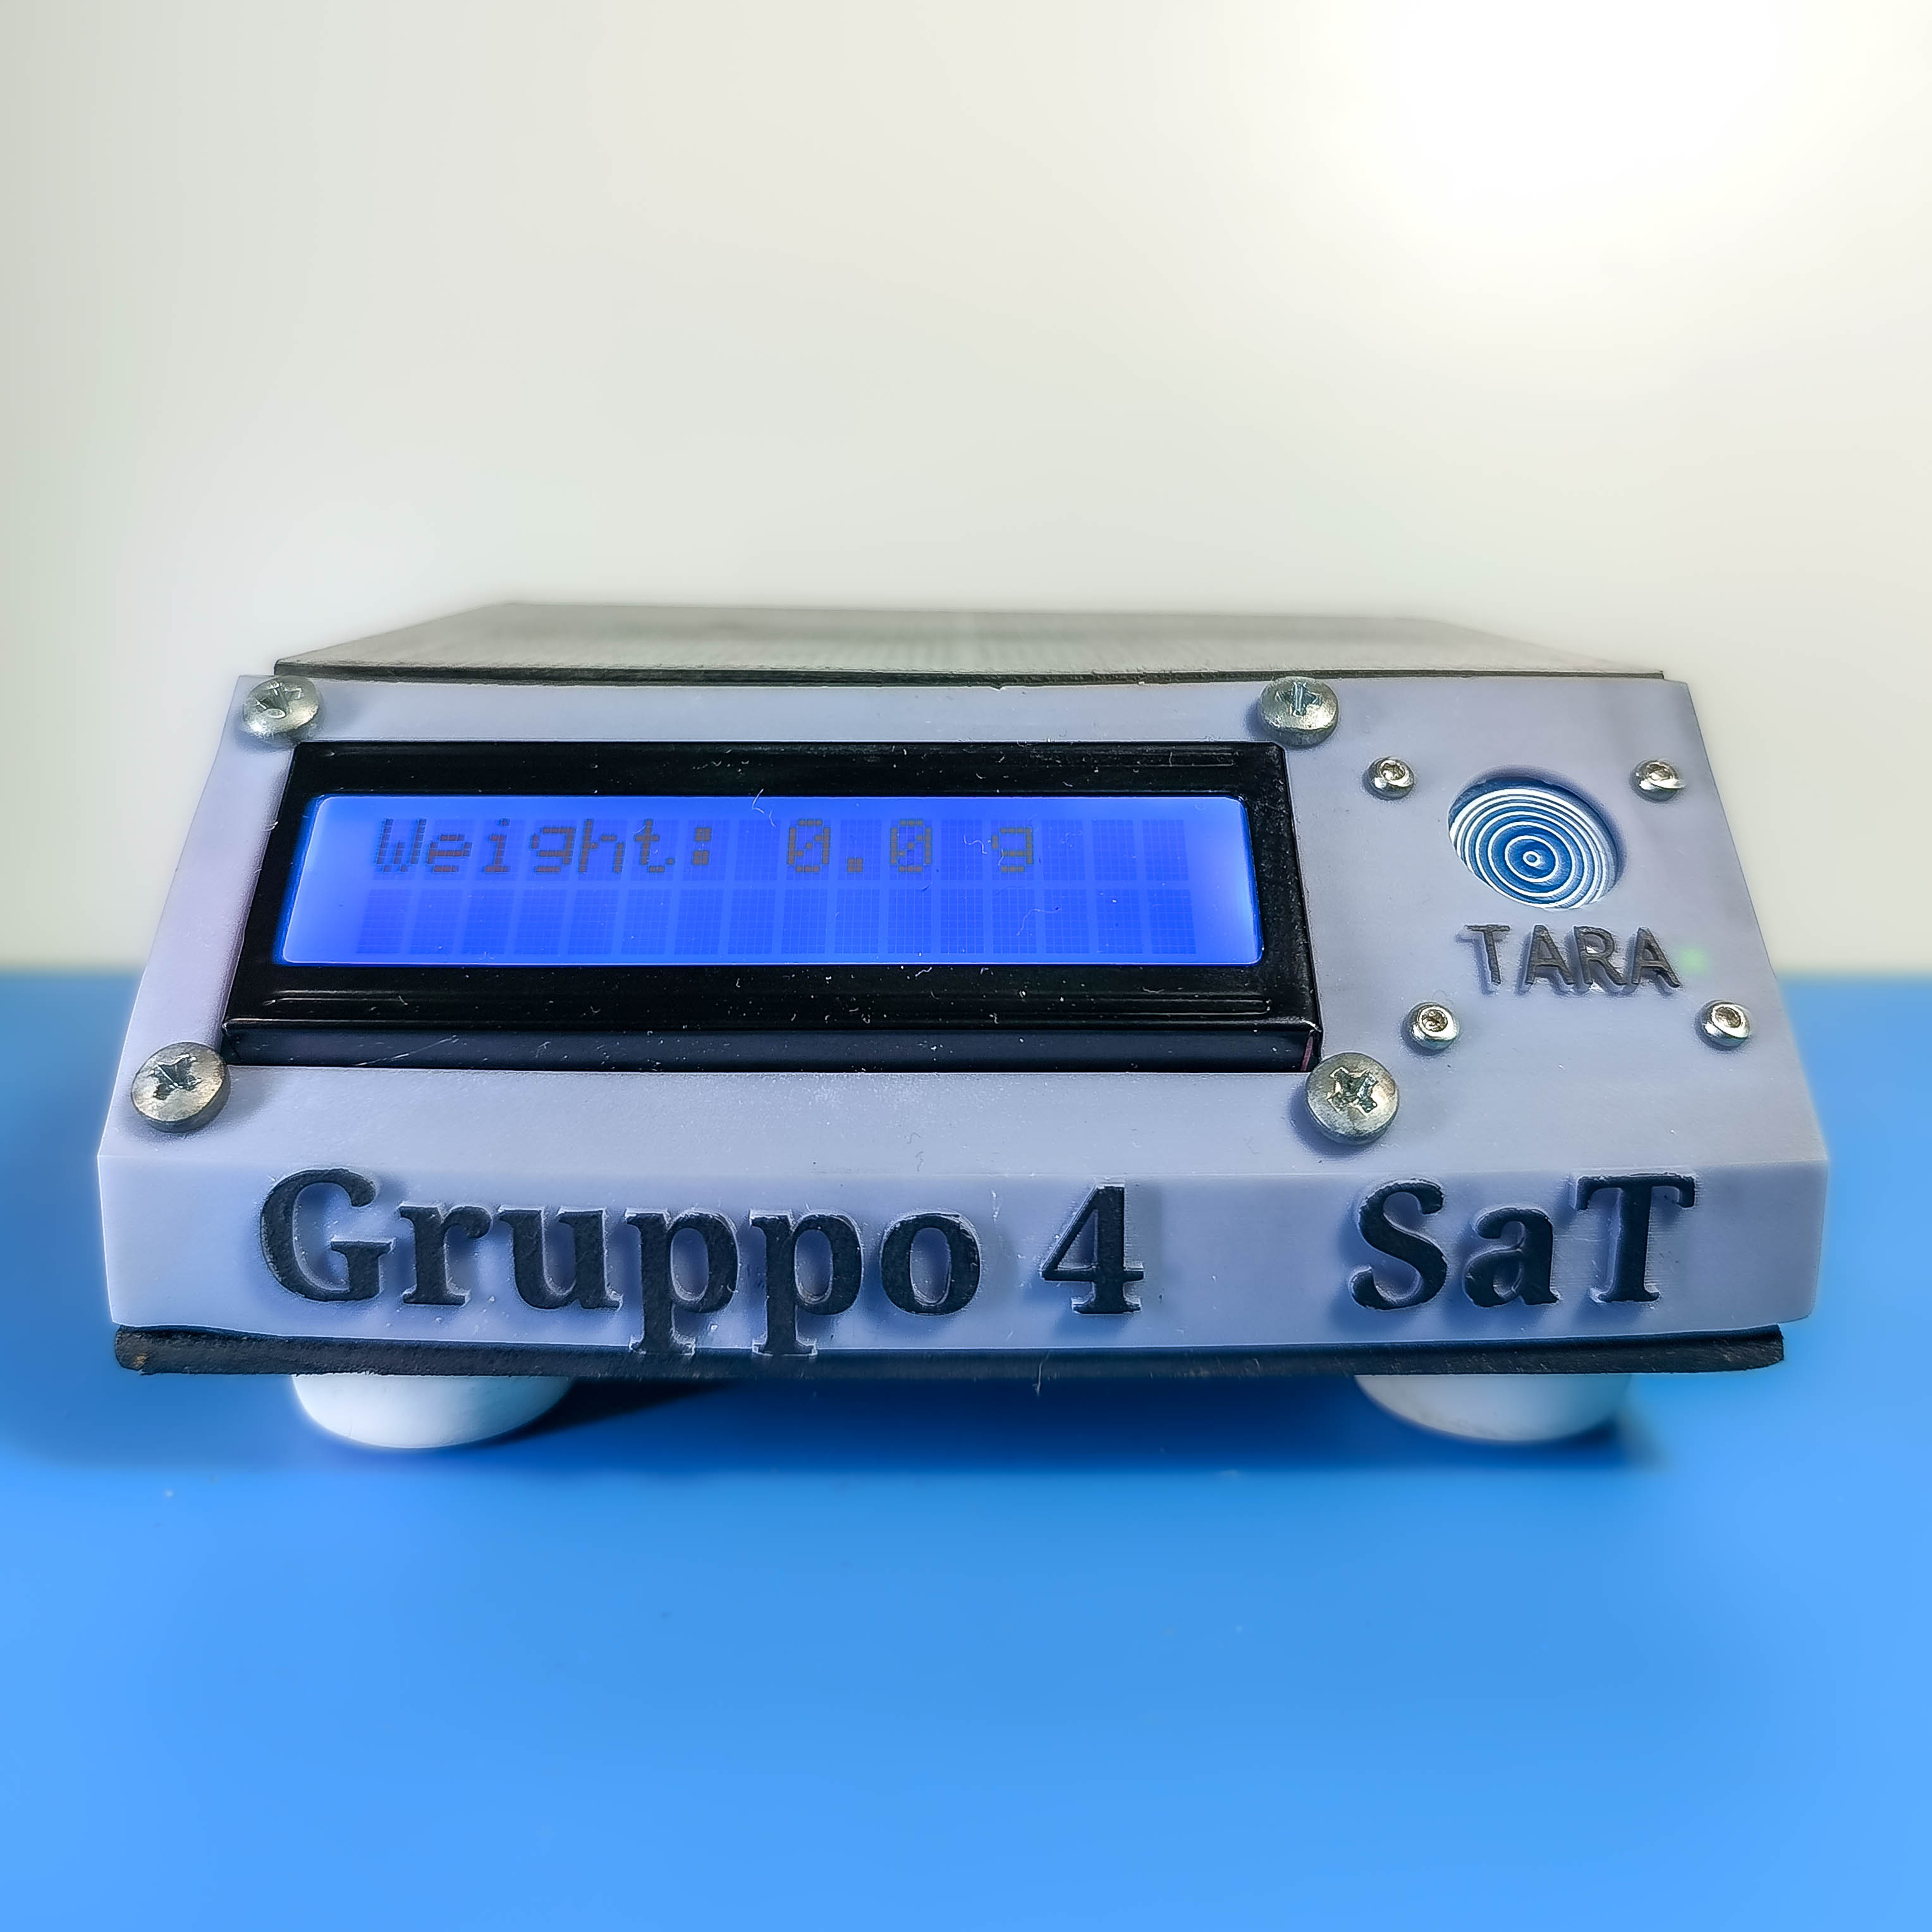
\includegraphics[width=0.6\textwidth]{medias/photos/front.jpg}
    \caption{Front view}
    \label{fig:immagine}
\end{figure}



\begin{figure}[ht]
\centering
\begin{minipage}{.5\textwidth} 
  \centering
  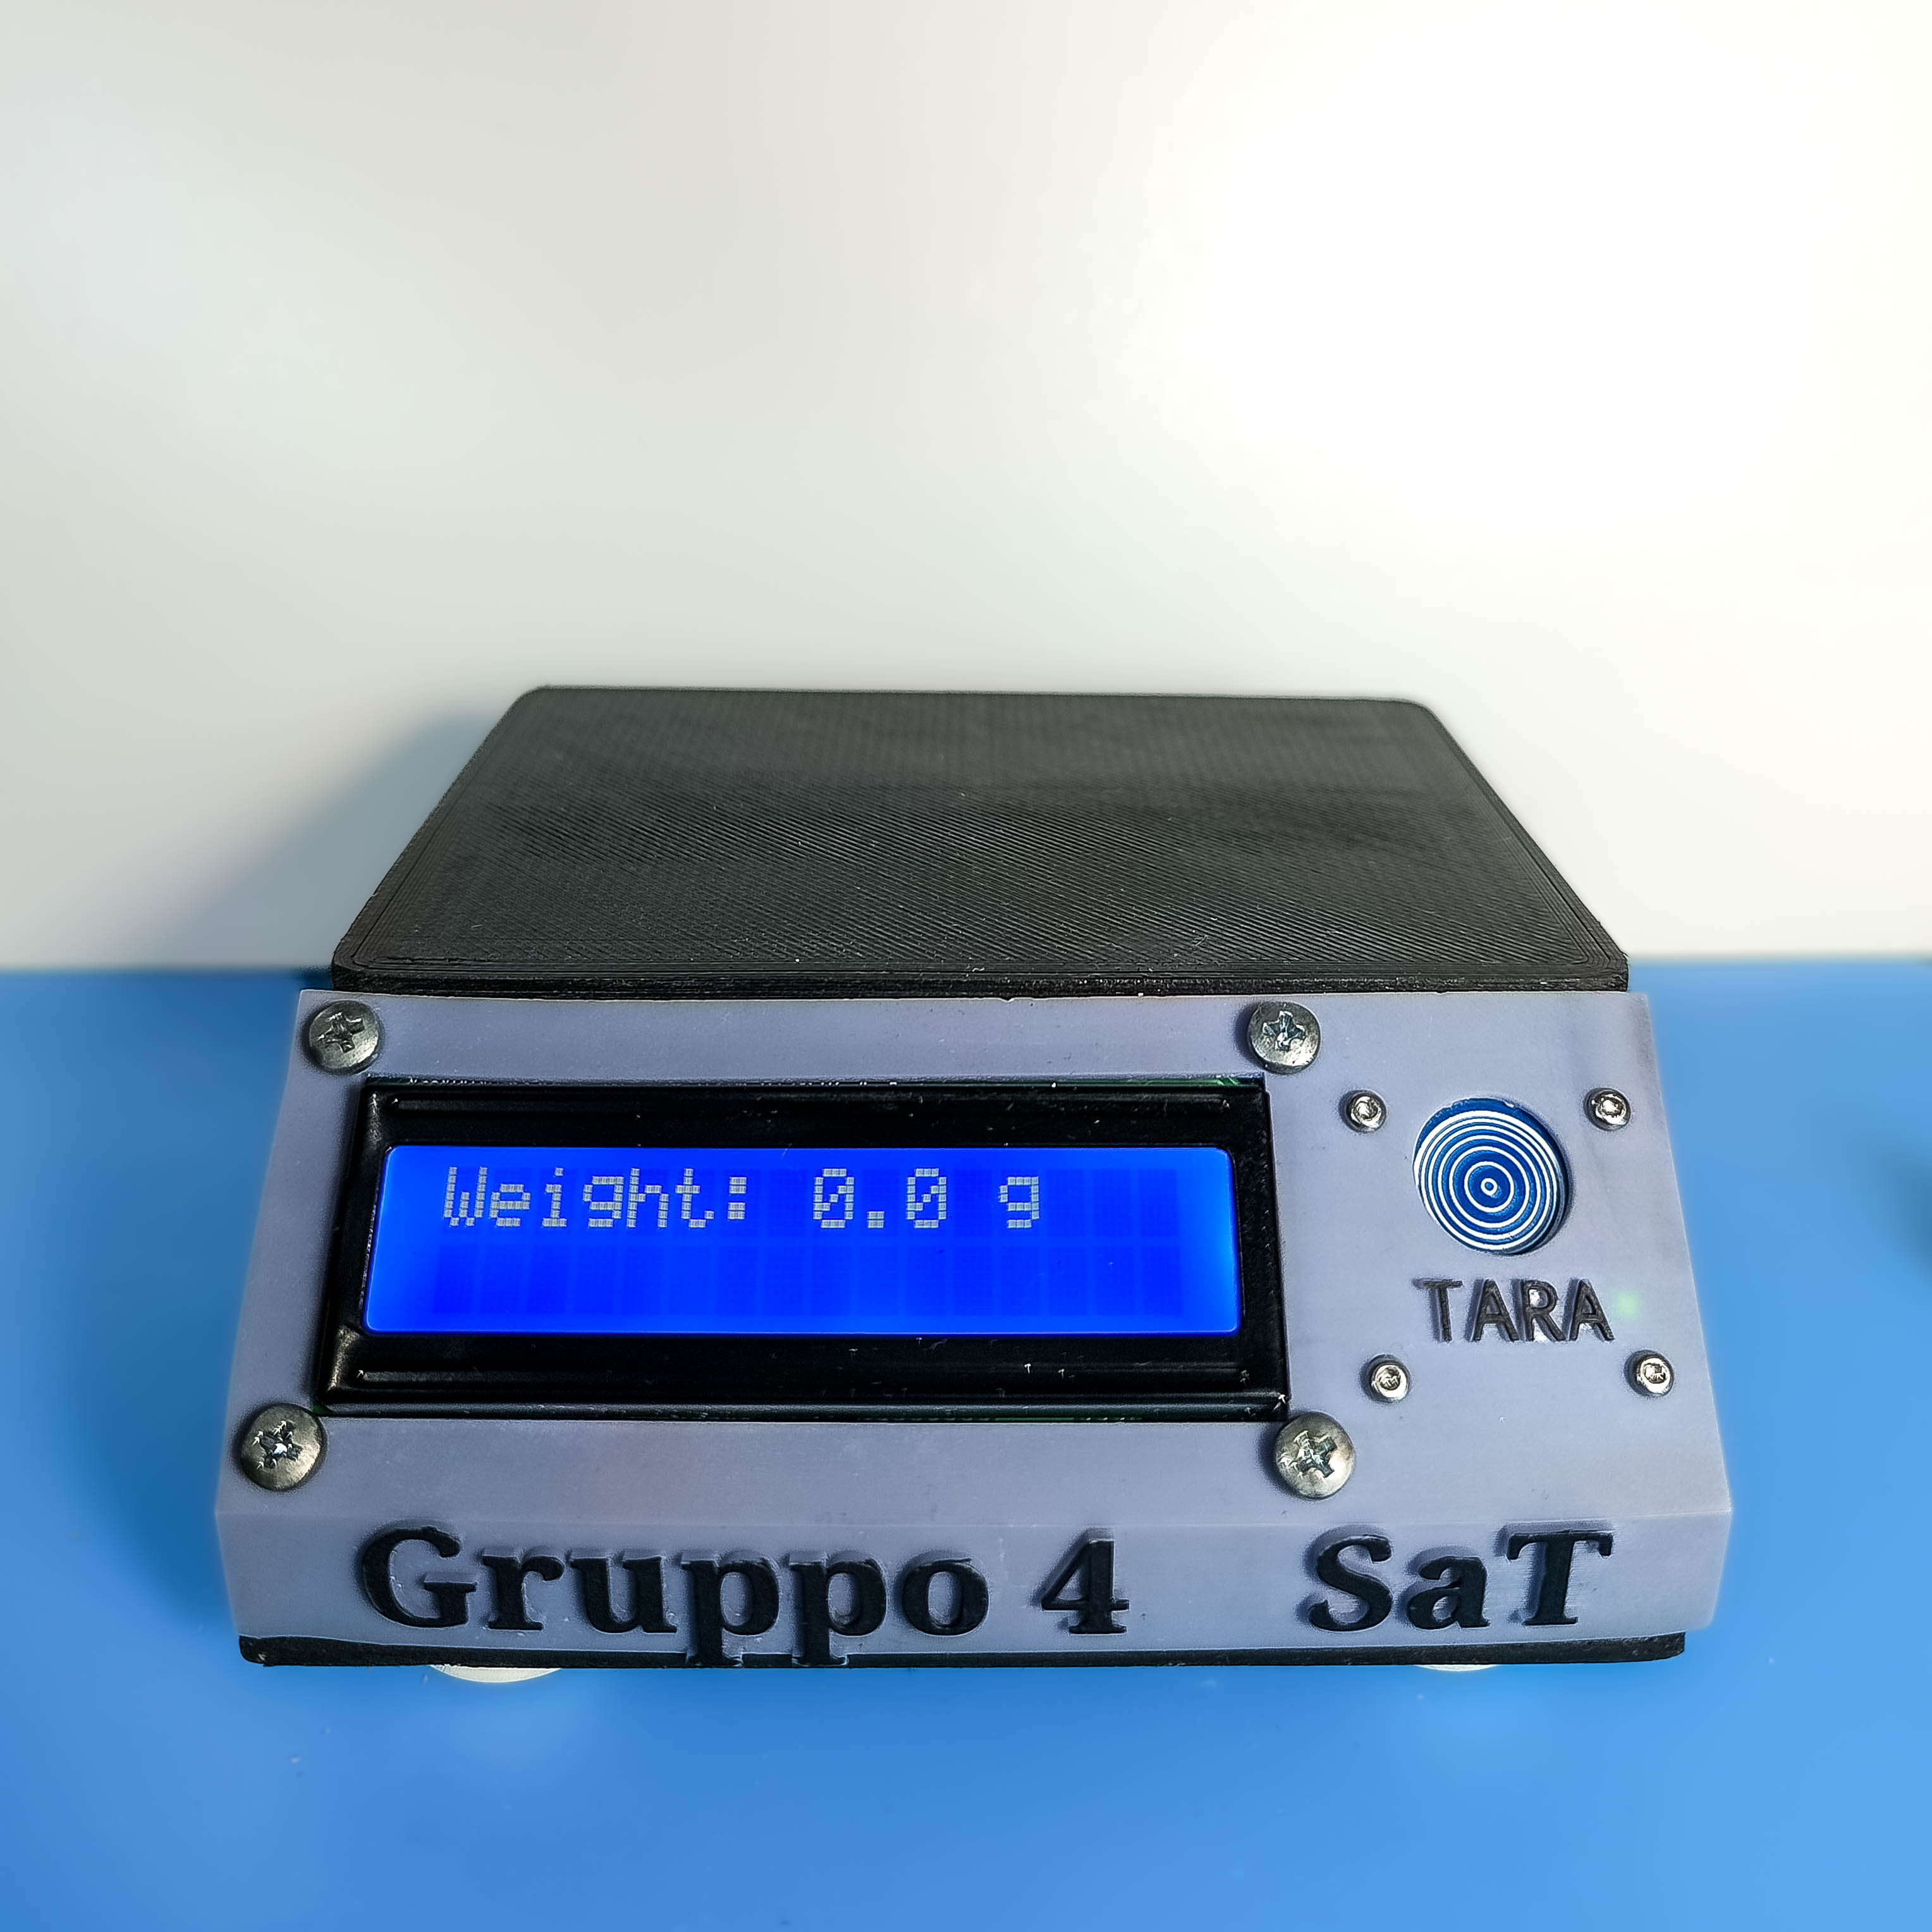
\includegraphics[width=.9\linewidth]{medias/photos/top.jpg}
  \caption{Top view}
  \label{fig:test1}
\end{minipage}%
\begin{minipage}{.5\textwidth} 
  \centering
  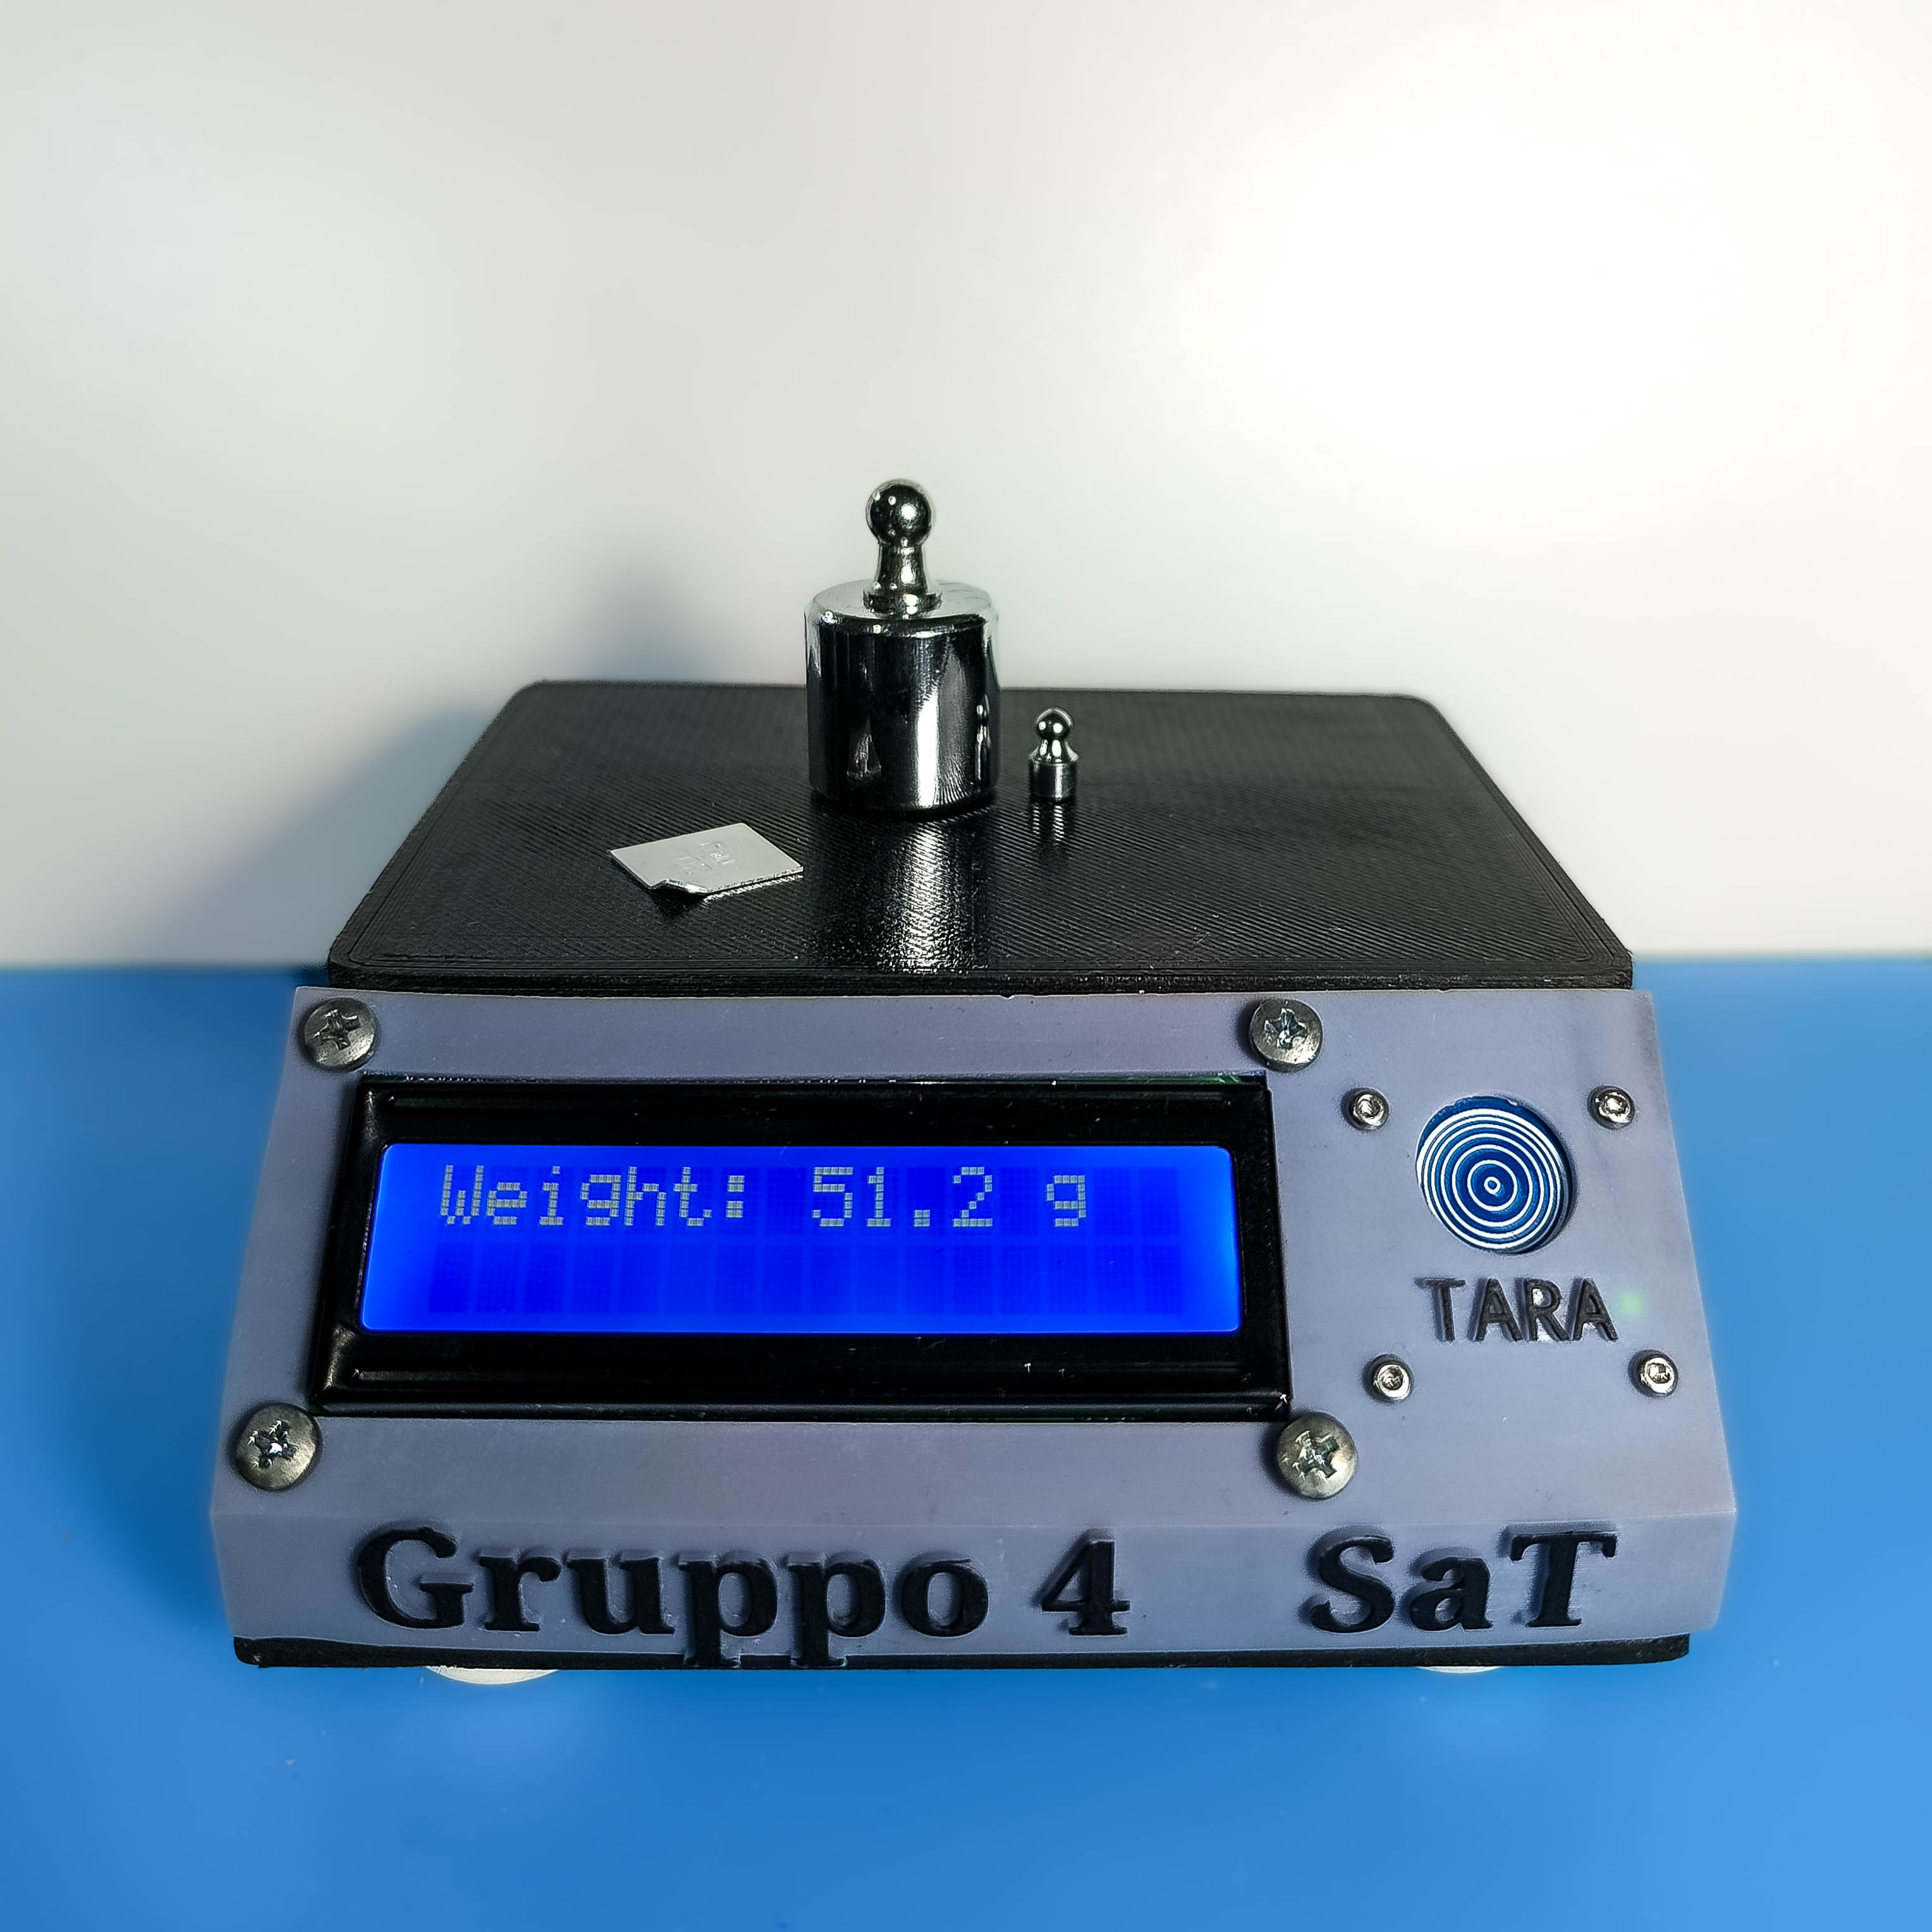
\includegraphics[width=.9\linewidth]{medias/photos/top2.jpg}
  \caption{Top view}
  \label{fig:test2}
\end{minipage}
\end{figure}


\begin{figure}[H]
    \centering
    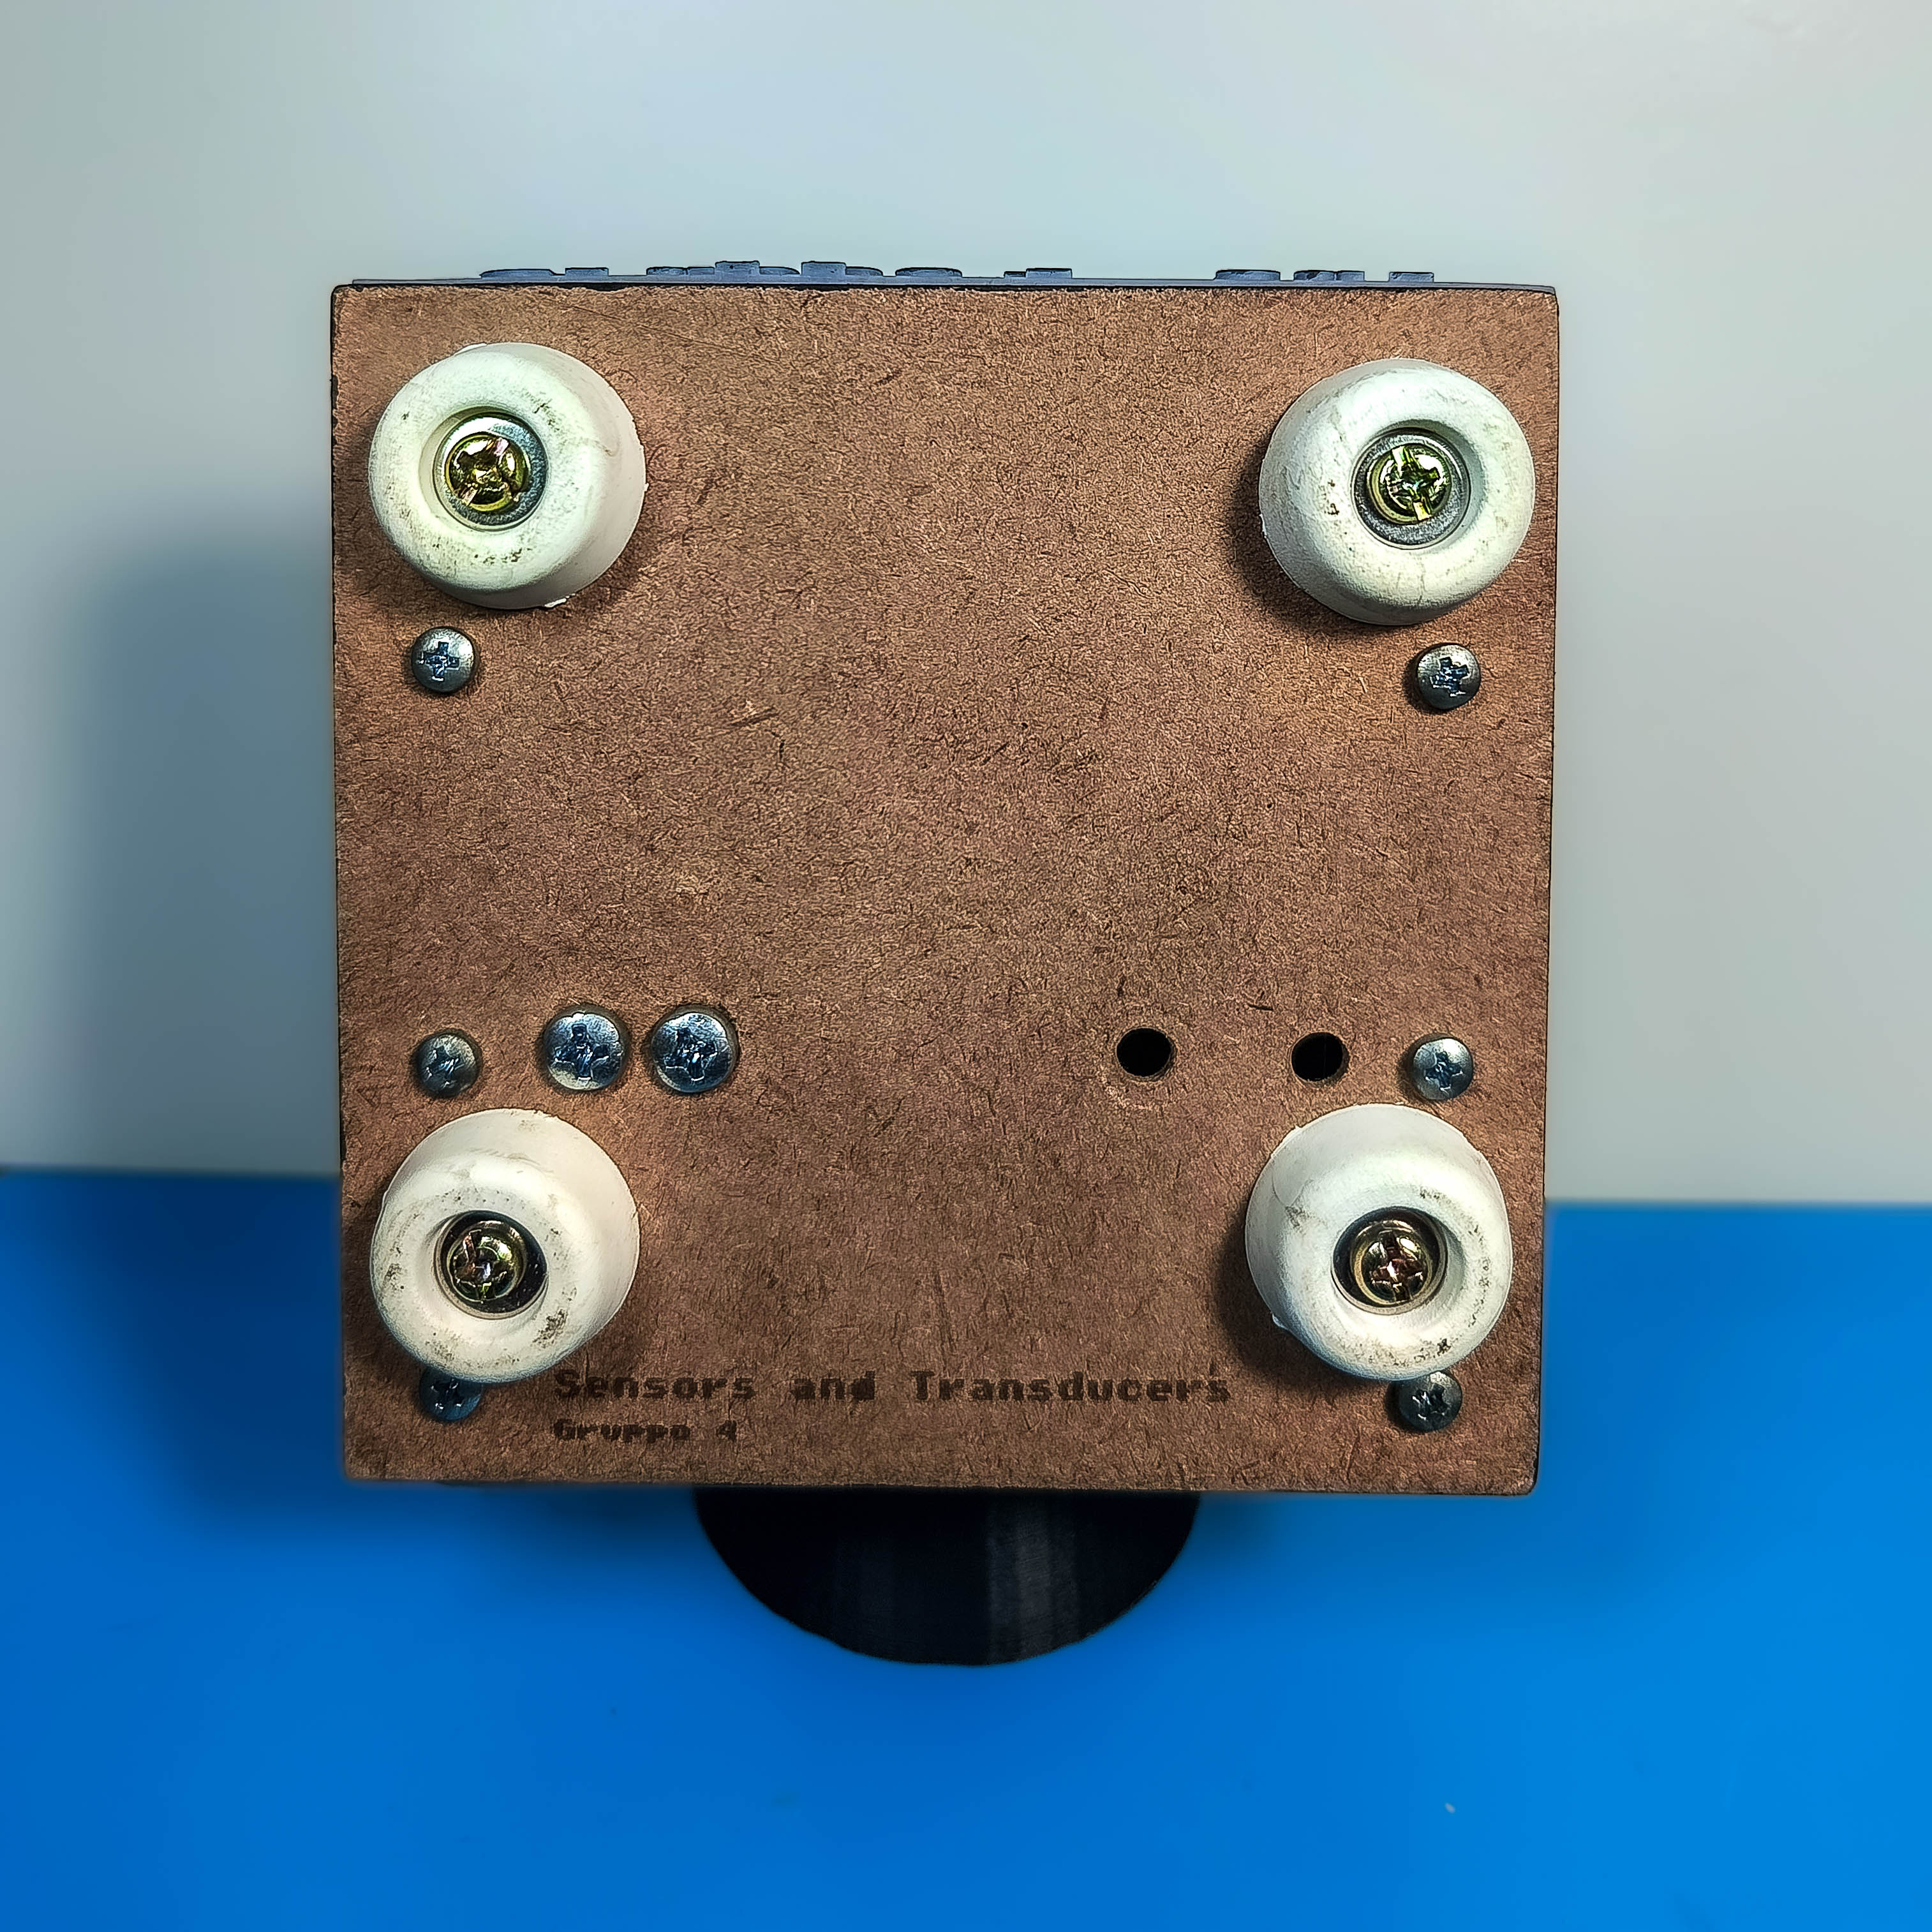
\includegraphics[width=0.65\textwidth]{medias/photos/bottom.jpg}
    \caption{Bottom view}
    \label{fig:immagine}
\end{figure}

\begin{figure}[ht]
\centering
\begin{minipage}{.5\textwidth} 
  \centering
  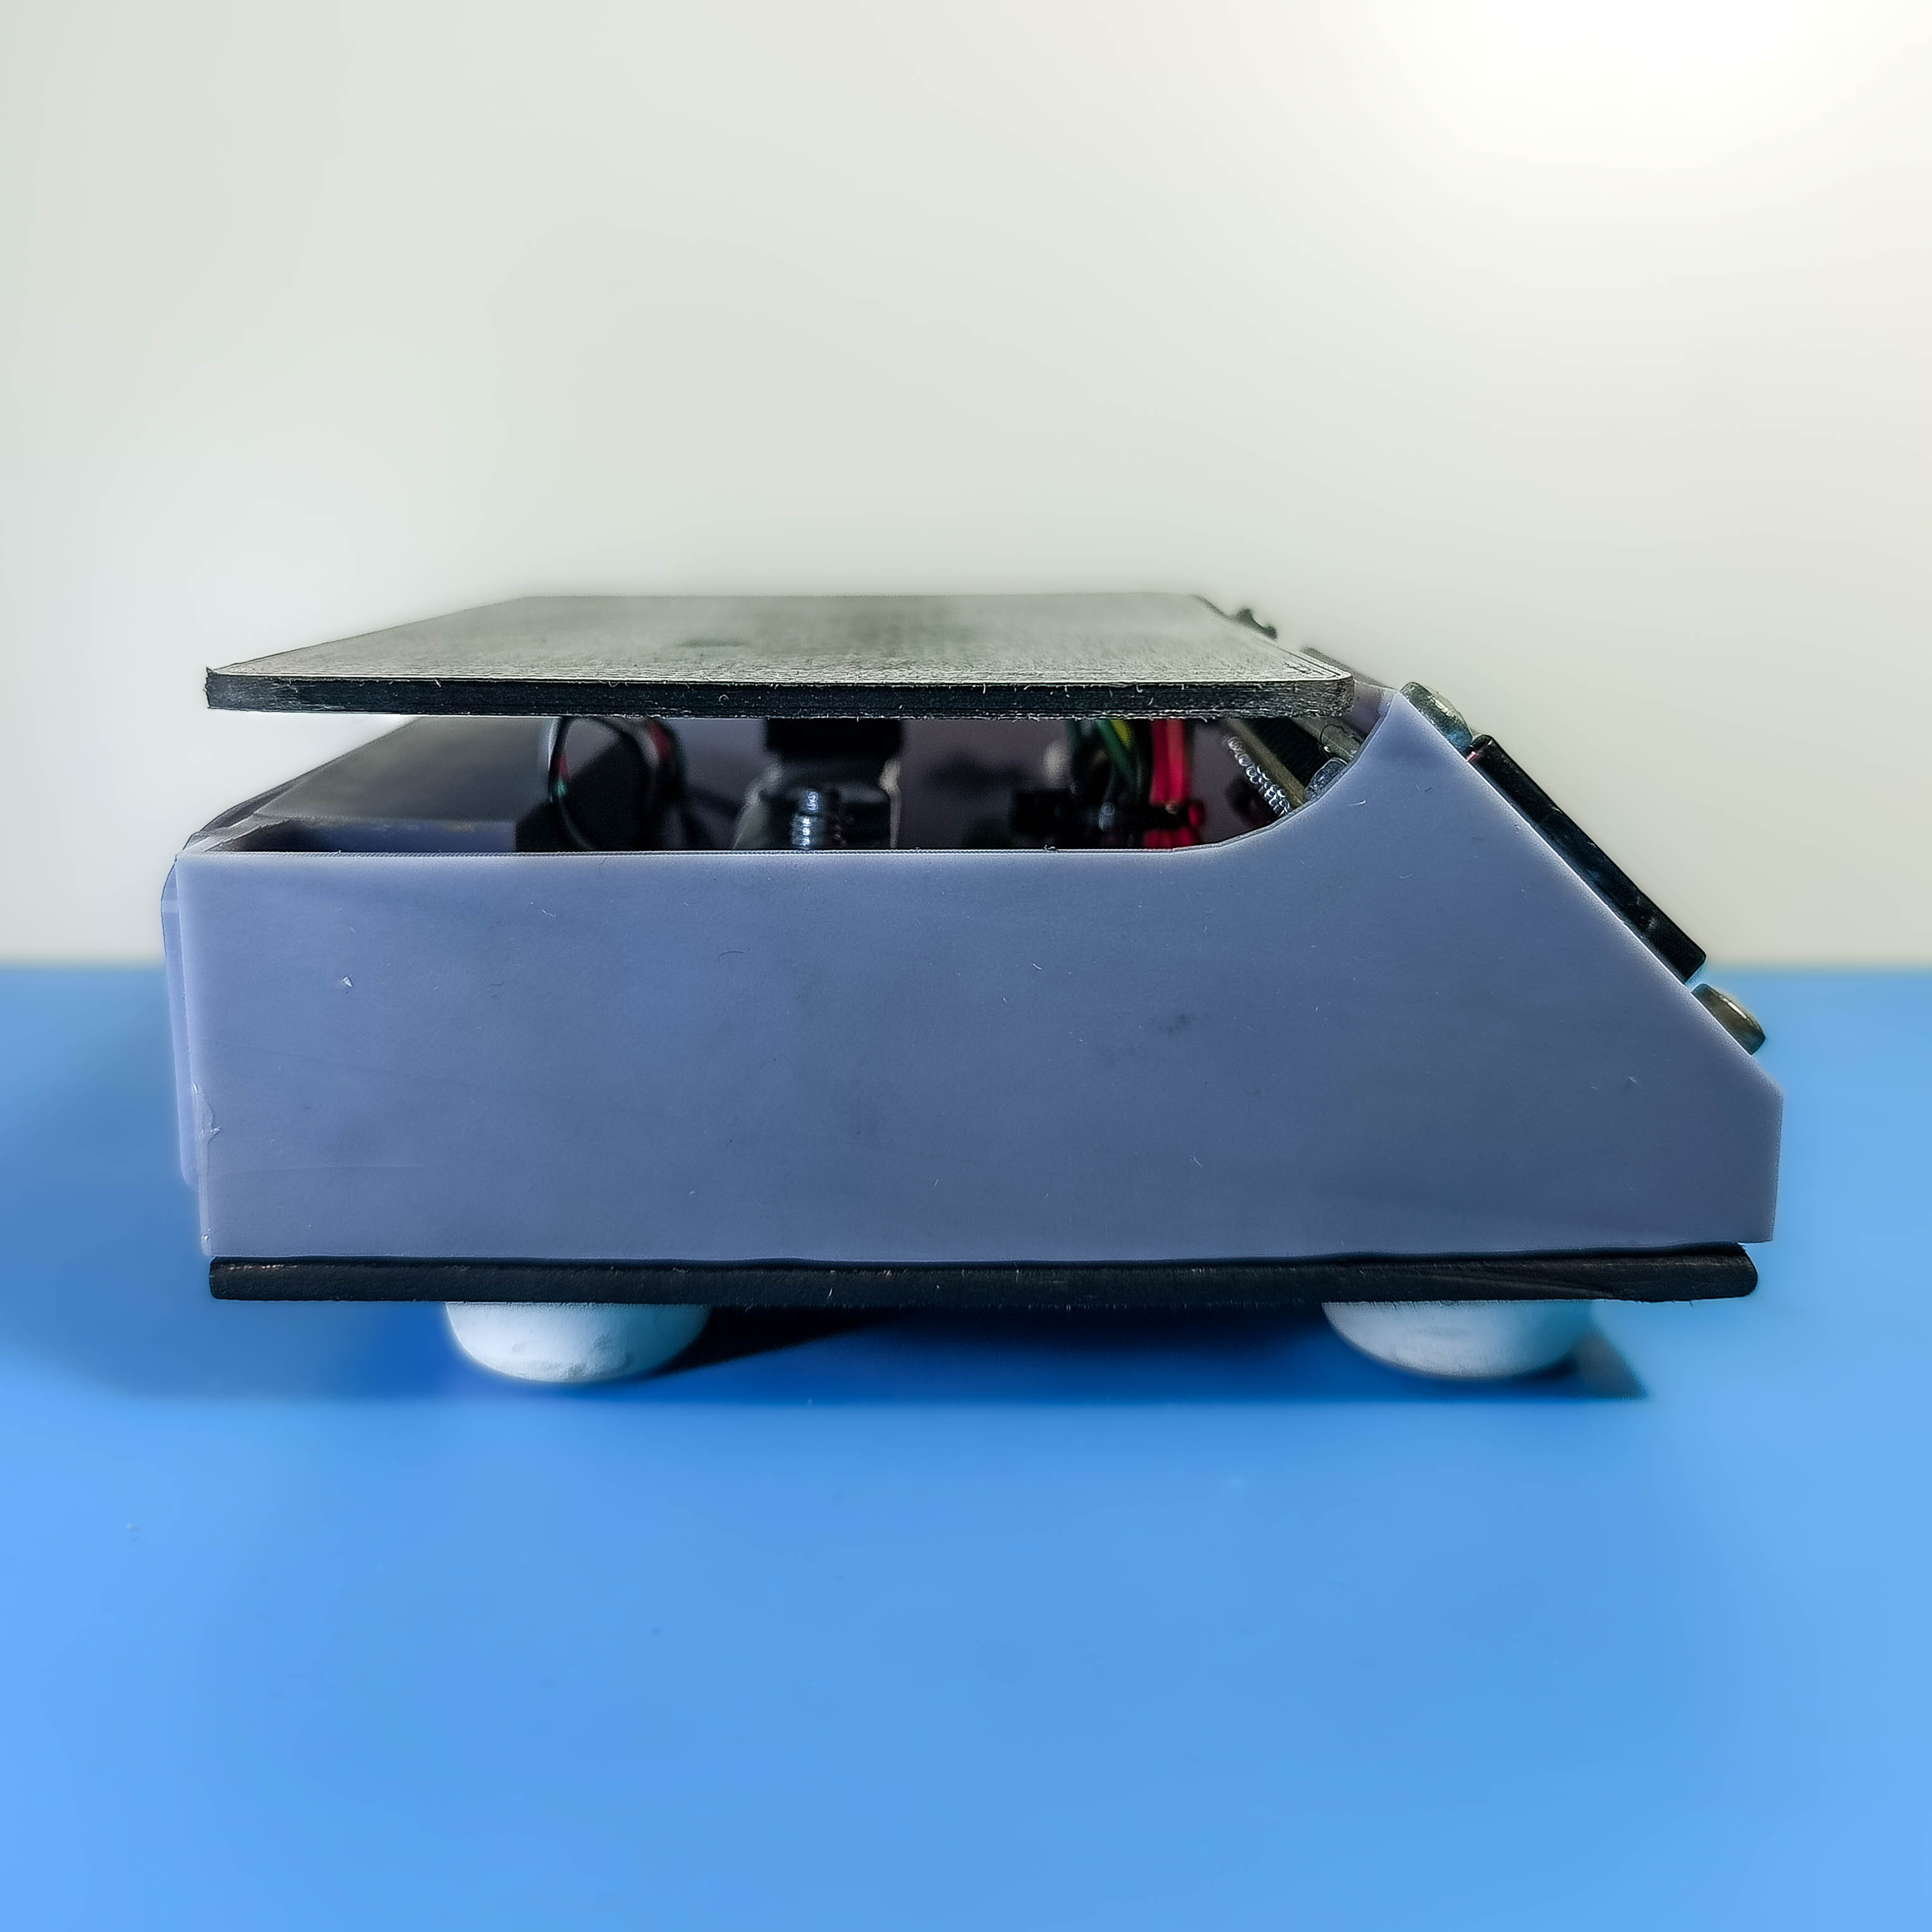
\includegraphics[width=.9\linewidth]{medias/photos/side1.jpg}
  \caption{Left side view}
  \label{fig:test1}
\end{minipage}%
\begin{minipage}{.5\textwidth} 
  \centering
  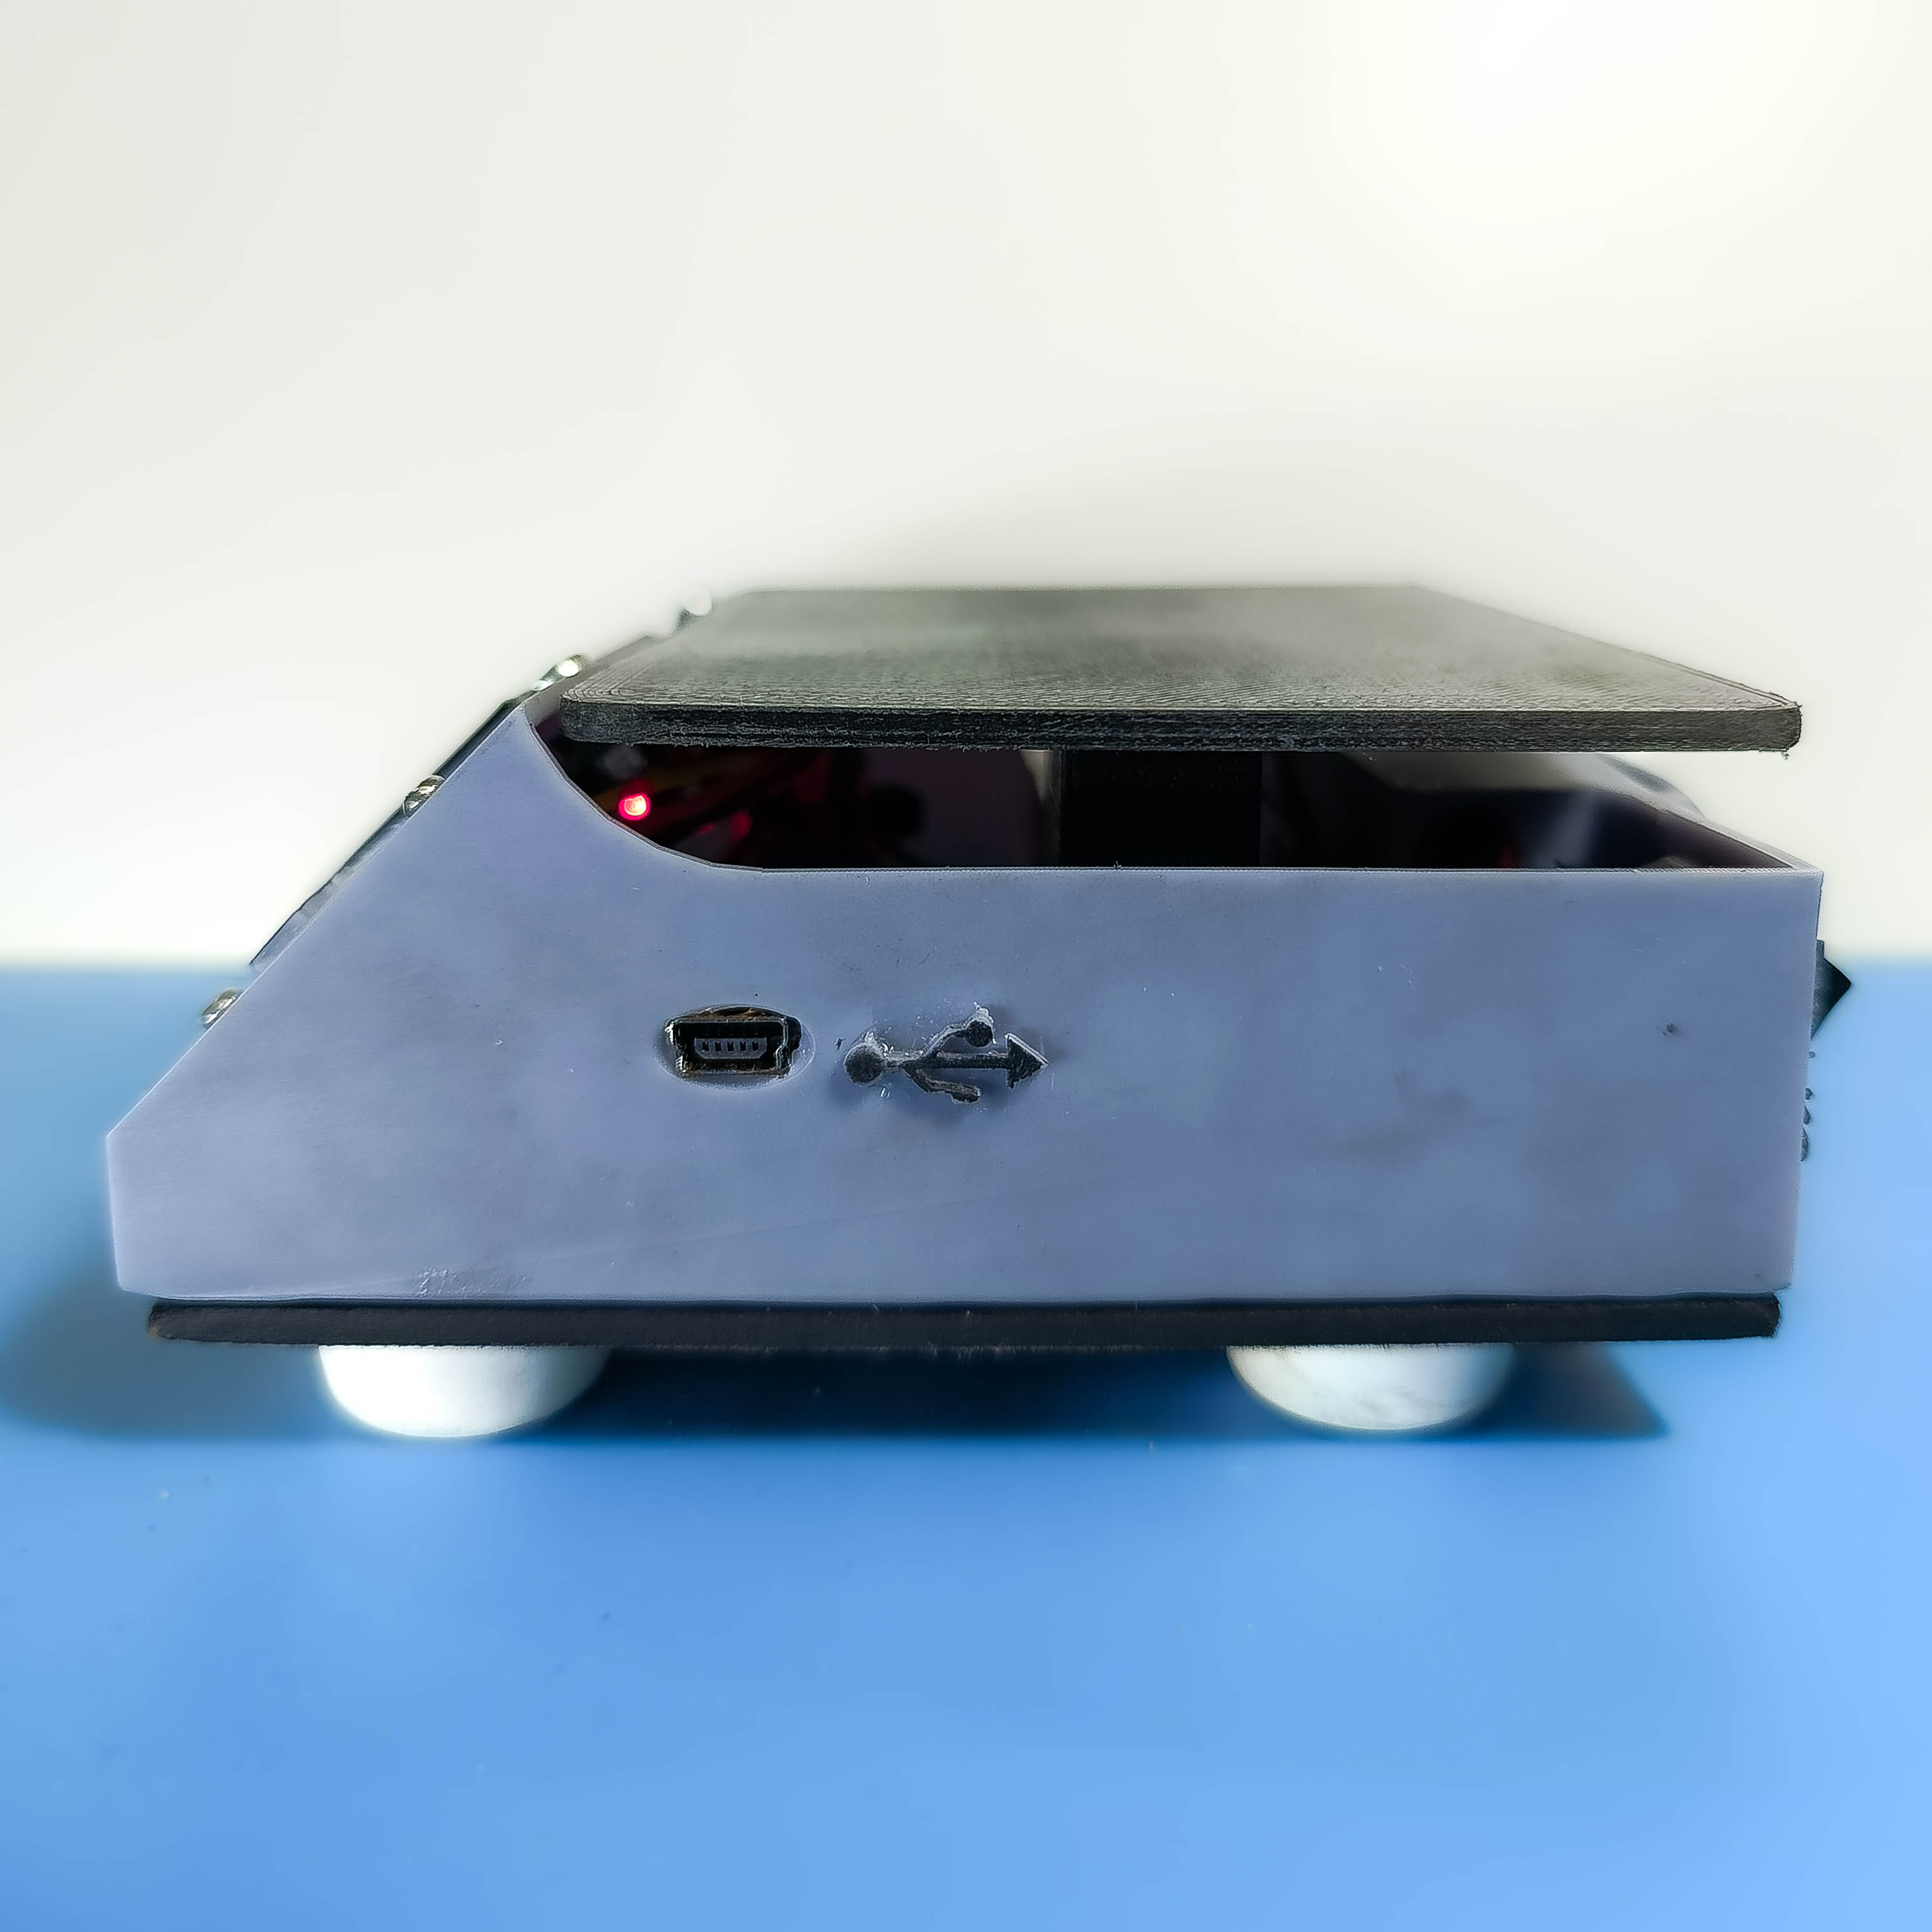
\includegraphics[width=.9\linewidth]{medias/photos/side2.jpg}
  \caption{Right side view}
  \label{fig:test2}
\end{minipage}
\end{figure}


\begin{figure}[H]
    \centering
    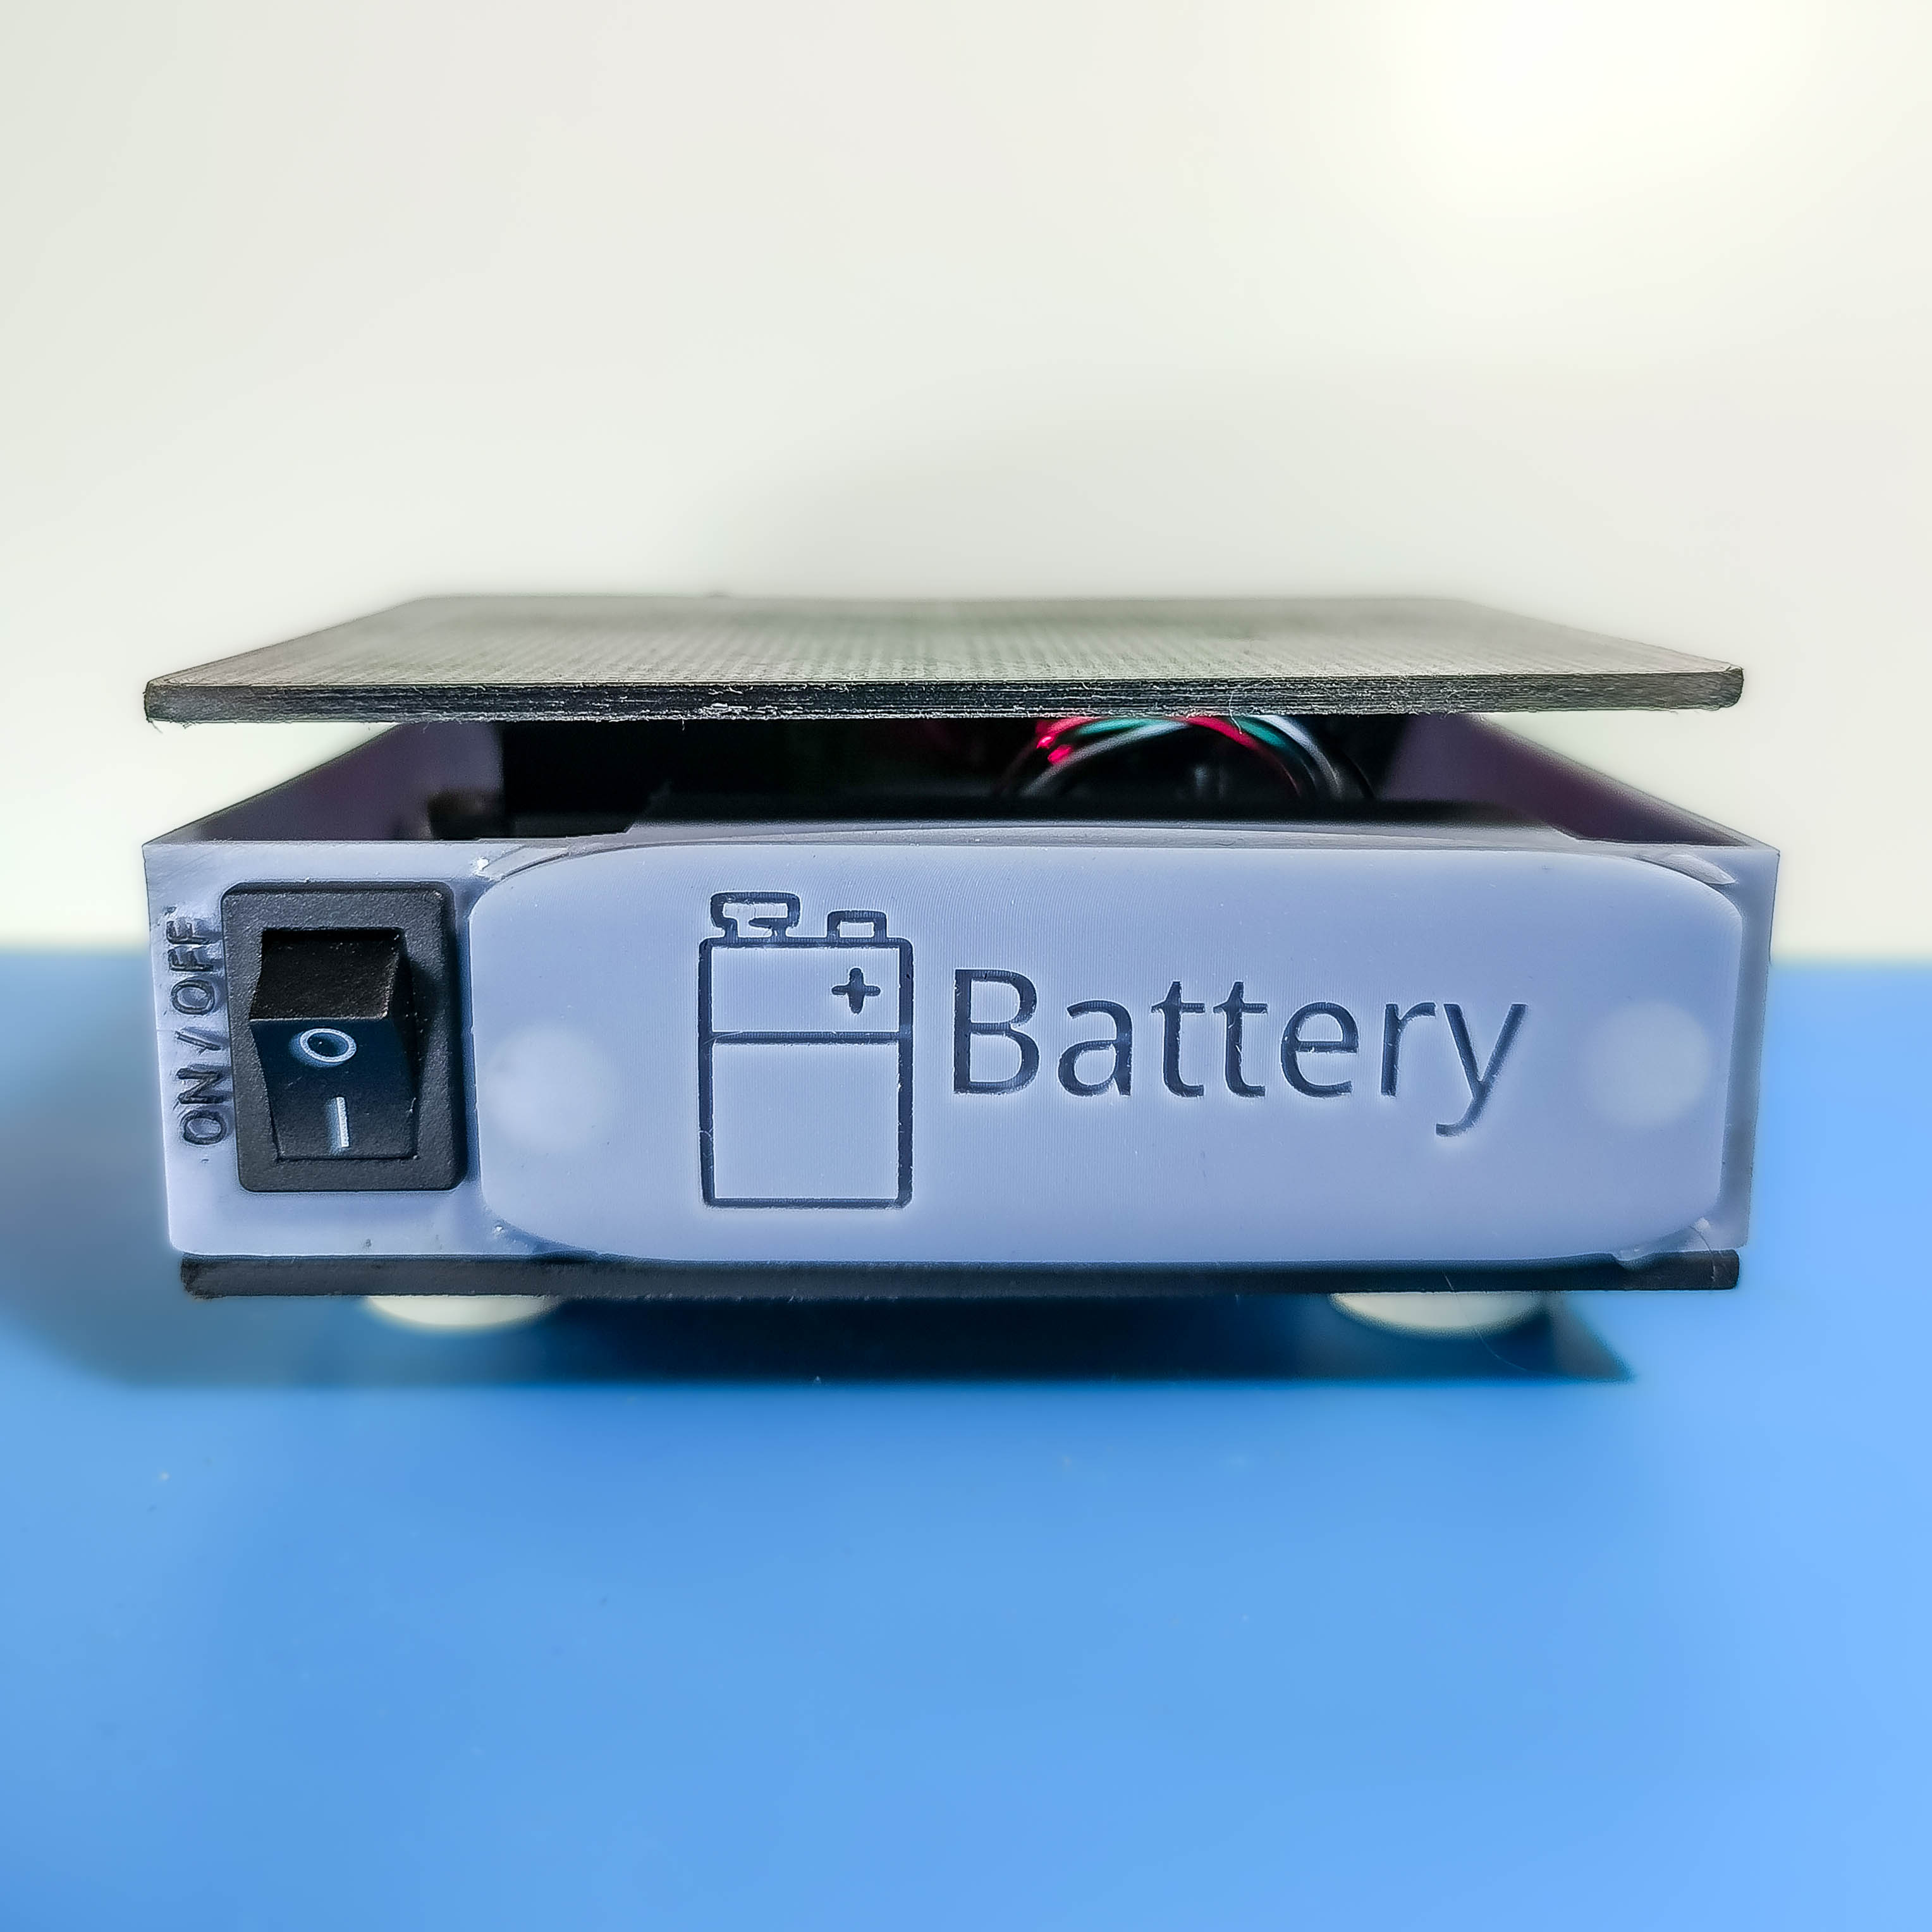
\includegraphics[width=0.65\textwidth]{medias/photos/back.jpg}
    \caption{Back view}
    \label{fig:immagine}
\end{figure}

\begin{figure}[H]
    \centering
    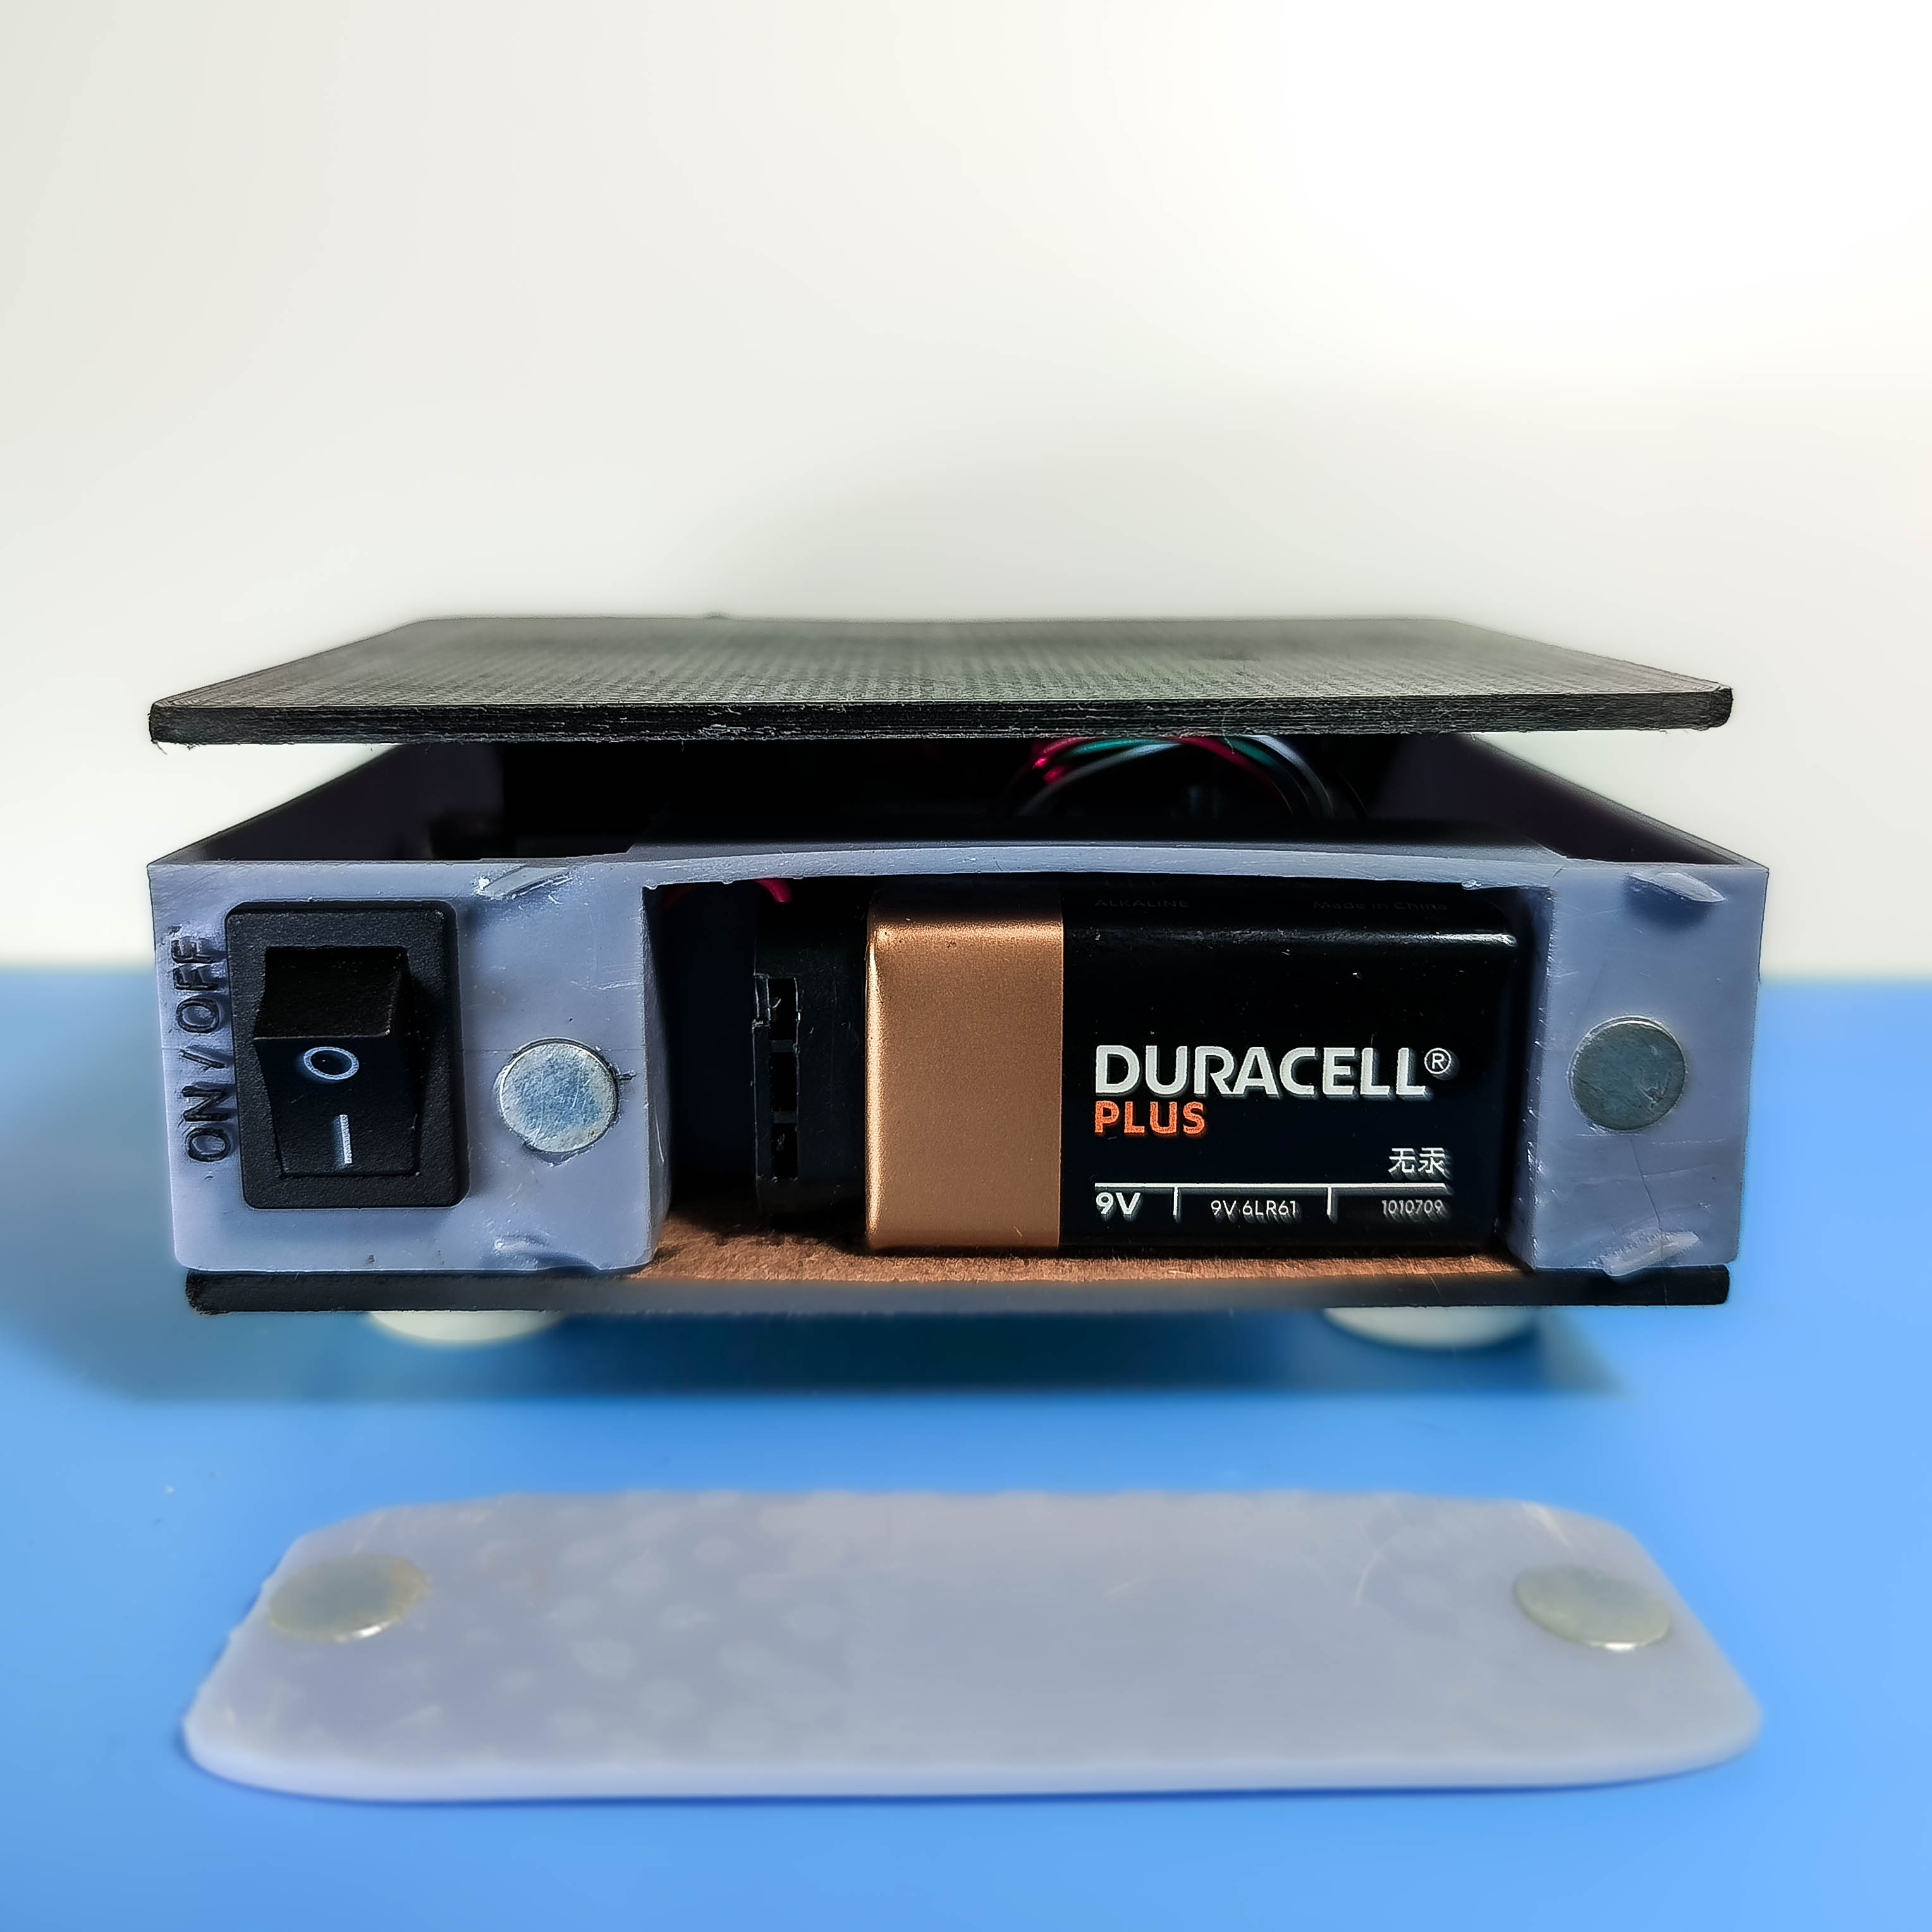
\includegraphics[width=0.65\textwidth]{medias/photos/back2.jpg}
    \caption{Back view}
    \label{fig:immagine}
\end{figure}